\section{Auswertung}

* Fortschritt in der Entwicklung

\subsection{Entwicklungsstand ITjobs}
\subsubsection*{Code-Qualität und Testabdeckung}
\subsubsection*{Diskussion}


\subsection{Code-Quality-Benchmark mit anderen Ruby-Projekten}

Um die Ergebnisse besser einordnen zu können, vergleichen wir die Ergebnisse aus den Code-Quality-Benchmark mit vergangenen Ruby-Projekten in der pludoni GmbH und mit bekannten Ruby/Rails-OpenSource Software.

Eine vollständige Metrik wie oben, war in vielen Fällen nicht möglich, da die Testwerkzeuge in vielen Fällen Inkompatibilitäten mit neueren Rubyversionen haben. Wir beschränken uns deshalb auf eine exemplarische Überblicksmetrik, bestehend aus:

\begin{description}
 \item[LOC] Anzahl der Quellcodezeilen, gemessen durch das Rails-Kommando "`rake stats"'. 
 \item[LOT] Anzahl der Quellcodezeilen aller Tests, gemessen durch das Rails-Kommando "`rake stats"'. 
 \item[LOT/TOC] Verhältnis aus Testzeilen und Quellcodezeilen
 \item[AVGCmplx] Durchschnittliche Komplexität aller Klassen, gemessen durch \textbf{Flog}\footnote{\url{https://github.com/seattlerb/flog}}. Flog besitzt ein eigenes Maß für Code-Komplexität. Es vergibt für jede Zuweisungen, Verzweigungen und Funktionsaufrufe unterschiedlich viele Punkte, und bildet so eine Summe per Funktion oder per Klasse. Dabei vergibt Flog besonders viele Punkte für schwer nachzuvollziehende Funktionsaufrufe, wie z.B. "`eval(string)"', welches einen String als Ruby-Code auswertet.
 \item[H5Cmplx] Komplexität der 5\% komplexesten Klassen, nach Flog
 \item[DSmell] Anzahl der Code-Smells nach Roodi. Beinhaltet u.a.: hohe Cyclomatische Komplexität in einer Methode (min. 4), lange Methoden, lange Parameterlisten, u.v.m.\footnote{\url{http://roodi.rubyforge.org/files/README_txt.html}}
 \item[DSmell/KLOC] Anzahl der Code-Smells nach Roodi pro tausend Codezeilen
 \item[CSmell] Anzahl der Code-Smells nach Reek. Diese beinhalten: Geringe Kohäsion, Duplikation, Control-Couple, Unkommunikativer Name von Methoden/Variablen/Parameter, verschachtelte Iteratoren, u.v.m  \footnote{\url{https://github.com/kevinrutherford/reek/wiki/Code-Smells}}
 \item[CSmell/KLOC] Anzahl der Code-Smells nach Reek pro tausend Codezeilen
\end{description}
%Die Tools Roodi und Reek messen beide gewisse \glossarpl{smell}, die sich zum Teil überdecken.







\subsubsection{Vergleich von IT-Jobs-und-Stellen mit eigenen Projekten}

Bisherige Projekte der pludoni GmbH und des Autors basierend auf Ruby/ Ruby on Rails
\begin{description}
 \item[feedmerger] Eine Rails-Anwendung zur Verwalten, Cachen, Filtern und Zusammenfügen von RSS und Atom-Feeds. Als OpenSource unter \url{https://github.com/zealot128/WenShanWenHai} zu finden.
 \item[pludonidb] Ist eine auf ActiveRecord basierende Bibliothek zur Anbindung der Datenbanken der Communityportale an Ruby-Skripte. Beinhaltet außerdem weitere Hilfsfunktionen für diese Domäne.
 \item[backlinks] Backlink und SEO-Success-Control ist eine Rails-2.3 Anwendung, zum Messen der sogenannten Backlinks\footnote{TODO} der Communitymitglieder und der Platzierung für relevante Sucheingaben in den großen Suchmaschinen (konkret: Welchen Platz hatte ein Communityportal an einem bestimmten Tag für "`it jobs dresden"', usw.) %TODO Verweis auf meinen Praktikumsbericht
 \item[lpp] Linkpartnerprogramm ist eine Studenteninitiative der TU Dresden, um ausländische Studenten mit deutschen Sprach- und Lernpartnern zusammenzubringen. Dazu wurde 2008 von einem Studententeam im Rahmen einer Semesterarbeit eine Rails-Webanwendung geschrieben. Der Autor dieser Arbeit war zwar nicht an der Entwicklung beteiligt, übernahm aber die Pflege und Weiterentwicklung selbiger.
\end{description}


\begin{table}[hbp]
 \caption{Vergleich von IT-jobs mit anderen Ruby Projekten des Autors/der pludoni GmbH}\label{table:cmpmy}
 \begin{center}
 
\begin{tabular}{|l|l|l|l|l|l|l|}
\hline\rowcolor{tableheadcolor}

Projekt&ItJobs&Backlinks&Feedmerger&SAnalyzer&Feedimport&PludoniDb\\
\hline
Technologie&Rails3&Rails2&Rails3&Rails3&Ruby&Ruby\\
\hline
Testverfahren&TDD&manuell&manuell&manuell&TDD&manuell\\
\hline
LOC&1570&1884&724&214&571&1933\\
\hline
LOT&1750&75&137&0&865&126\\
\hline
LOT/LOC&1.11&0.04&0.19&0.00&1.51&0.07\\
\hline
AVGCmplx&8.00&19.90&10.50&14.80&16.80&13.70\\
\hline
H5Cmplx&43.80&70.60&26.90&39.70&25.10&113.20\\
\hline
DSemll&11&69&11&11&8&25\\
\hline
DSmell/KLOC&7.00&36.60&15.20&51.40&14.00&12.90\\
\hline
CSmell&53&152&52&13&28&113\\
\hline
CSmell/KLOC&33.80&80.70&71.80&60.70&49.00&58.50\\
\hline
\end{tabular}
\end{center}

\end{table}


\subsubsection{Vergleich von IT-Jobs-und-Stellen mit anderen Rails Projekten}
Weiterhin wird das Projekt mit folgenden beliebten Webprojekten, welche ebenfalls auf Ruby on Rails basieren, verglichen:
\begin{description}
 \item[diaspora] Ist ein verteiltes soziales Netzwerk. \\
 Code: \url{https://github.com/diaspora/diaspora}
 \item[bucketwise] ist ein web-basierter persönlicher Finanzmanager mit Budgetierung nach dem Briefumschlagsystem\\
 Code: \url{https://github.com/jamis/bucketwise}
 \item[chiliproject] Ist ein Fork\footnote{In der (Open-Source) Software-Entwicklung ist ein Fork eine legale Kopie eines bestehendes Software-Produktes, um von nun an eine unabhängige Entwicklung zu betreiben} des sehr beliebten Bugtrackers Redmine\footnote{https://github.com/edavis10/redmine}. Statt des originalen Redmines wurde dieser Fork genommen, da er eine neuere Codebasis hat\\
 Code: \url{https://github.com/chiliproject/chiliproject}
 \item[railscast] Ist der Code der Website \url{http://www.railscasts.com}, in welche allwöchentlich ein Screencast zum Thema Ruby und Rails veröffentlich wird (bis dato 283 Episoden).\\
 Code: \url{https://github.com/ryanb/railscasts} 
 \item[ActiveSupport] Beinhaltet Hilfsklassen und Erweiterungen der Standardbibliothek für \glossar{rails}. Kernbestandteil von Ruby on Rails \\
 Code: \url{https://github.com/rails/rails.git}
 \item[ActionPack]  ist Framework um Anfragen und Antworten eines Webservers zu verarbeiten und ist ein weiterer Kernbestandteil von Rails.\\
 Code: \url{https://github.com/rails/rails.git}
\end{description}

\begin{table}[hbp]
 \caption{Vergleich von IT-jobs mit Ruby/Rails Projekten aus der Community}\label{table:cmpother}
 \begin{tabular}{|p{1.8cm}|l|l|l|l|l|l|l|l|}
\hline \rowcolor{tableheadcolor}
 Projekt&itjobs&bucket&lpp&chili&aPack&aSupport&diaspora&rCasts\\
\hline
Technologie&Rails3&Rails2&Rails1&Rails2&Rails3&Rails3&Rails3&Rails3\\
\hline
LOC&1570&1979&7116&21201&12995&9407&7466&653\\
\hline
LOT&1750&1684&1557&20127&32570&13590&10072&748\\
\hline
LOT/LOC&1.11&0.85&0.22&0.95&2.51&1.44&1.35&1.15\\
\hline
AVGCmplx&8.00&12.80&17.10&19.10&11.10&10.90&13.10&11.00\\
\hline
H5Cmplx&43.80&32.20&181.80&84.40&64.00&47.90&54.00&34.60\\
\hline
DSmell&11&37&250&651&370&166&99&2\\
\hline
DSmell\newline~/KLOC&7.00&18.70&35.10&30.70&28.50&17.60&13.30&3.10\\
\hline
CSmell&53&129&386&1535&982&291&324&42\\
\hline
CSmell\newline~/KLOC&33.80&65.20&54.20&72.40&75.60&30.90&43.40&64.30\\
\hline
\end{tabular}
\end{table}

TODO Auswertung

\begin{figure}[hp]
 \centering
 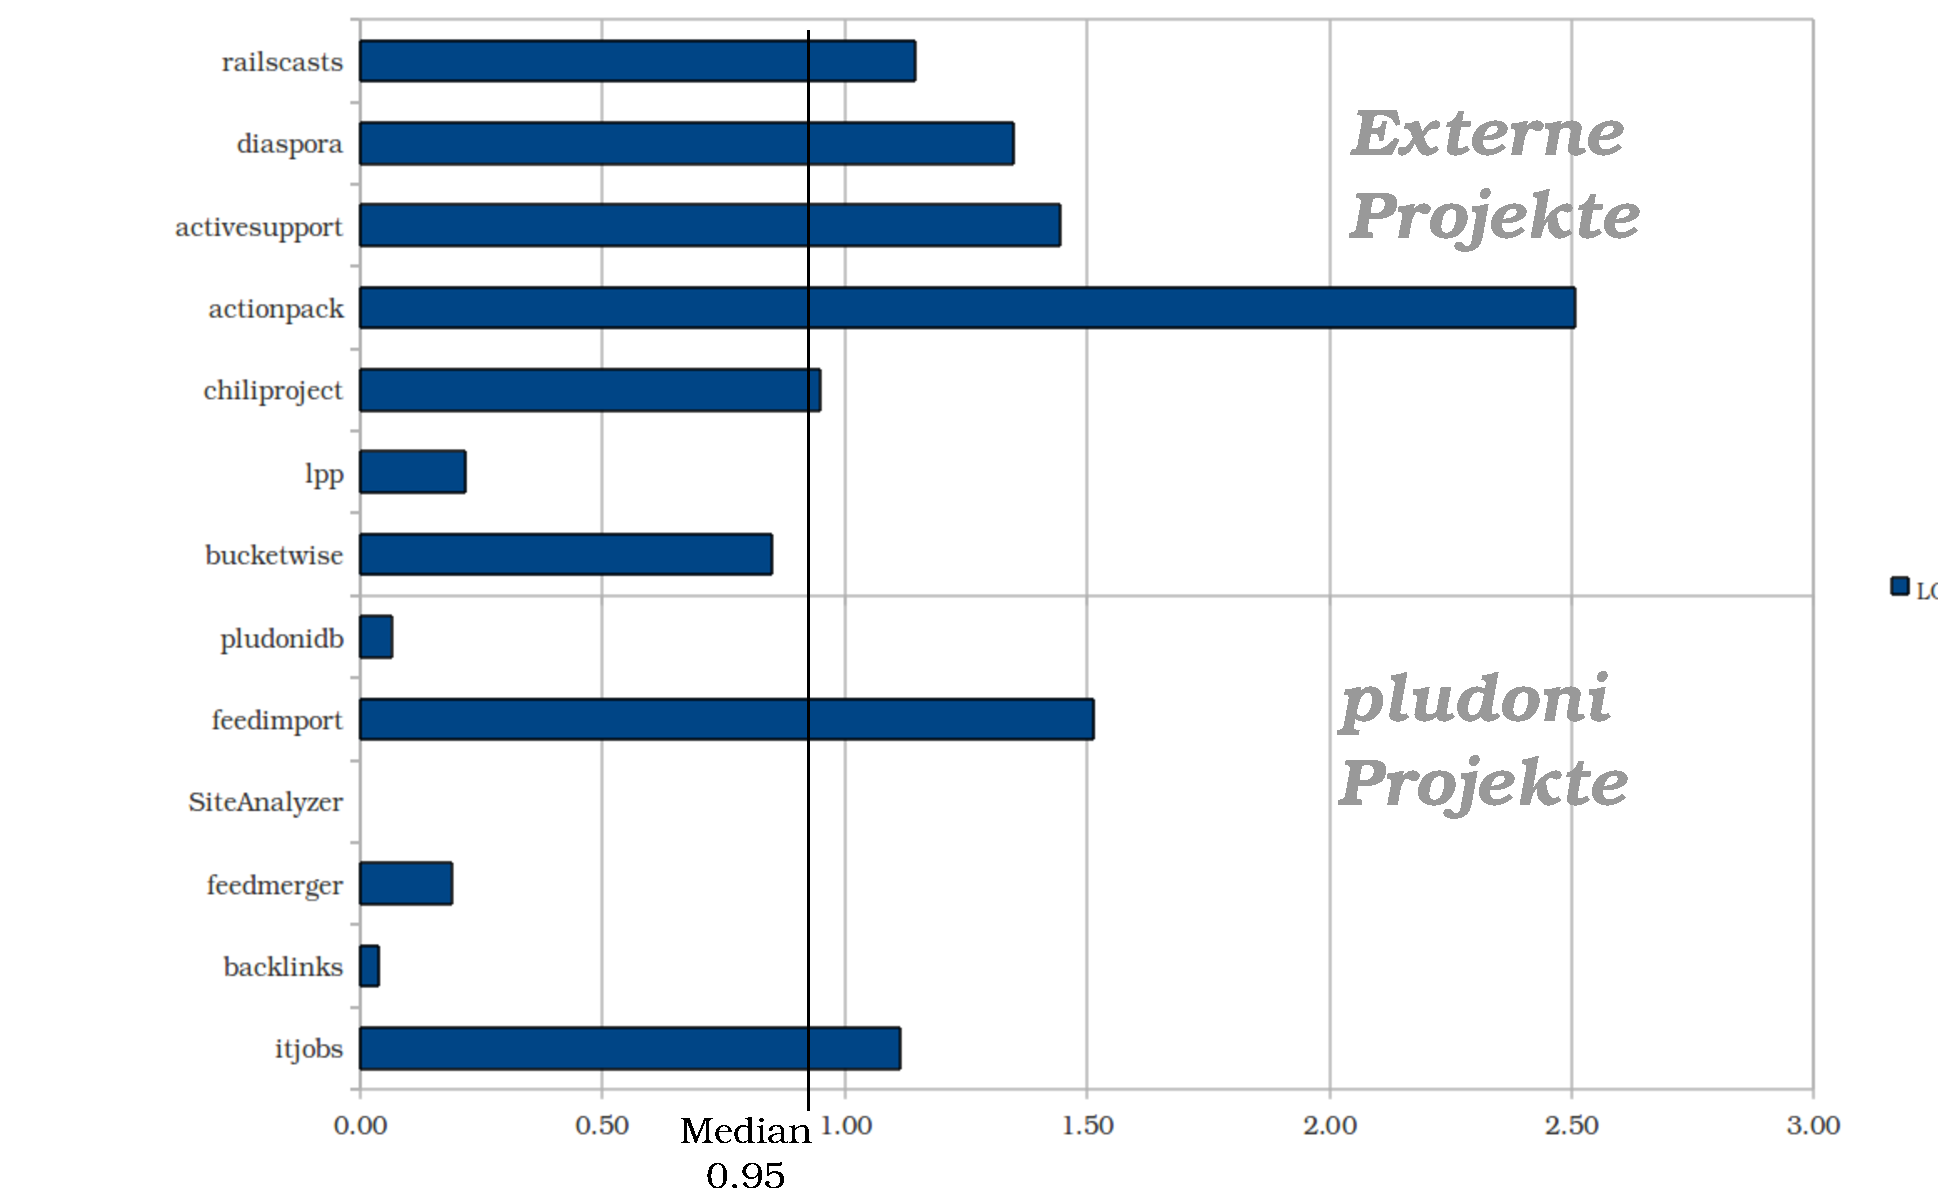
\includegraphics[width=\linewidth]{./diagrams/cpm-lotloc.pdf}
 % cpm-lotloc.pdf: 930x574 pixel, 72dpi, 32.81x20.25 cm, bb=0 0 930 574
 \caption{Vergleich des Verhältnisses aus Anzahl Testcodezeilen / Anzahl Codezeilen}
 \label{fig:cpm-complex}
\end{figure}

\begin{figure}[hp]
 \centering
 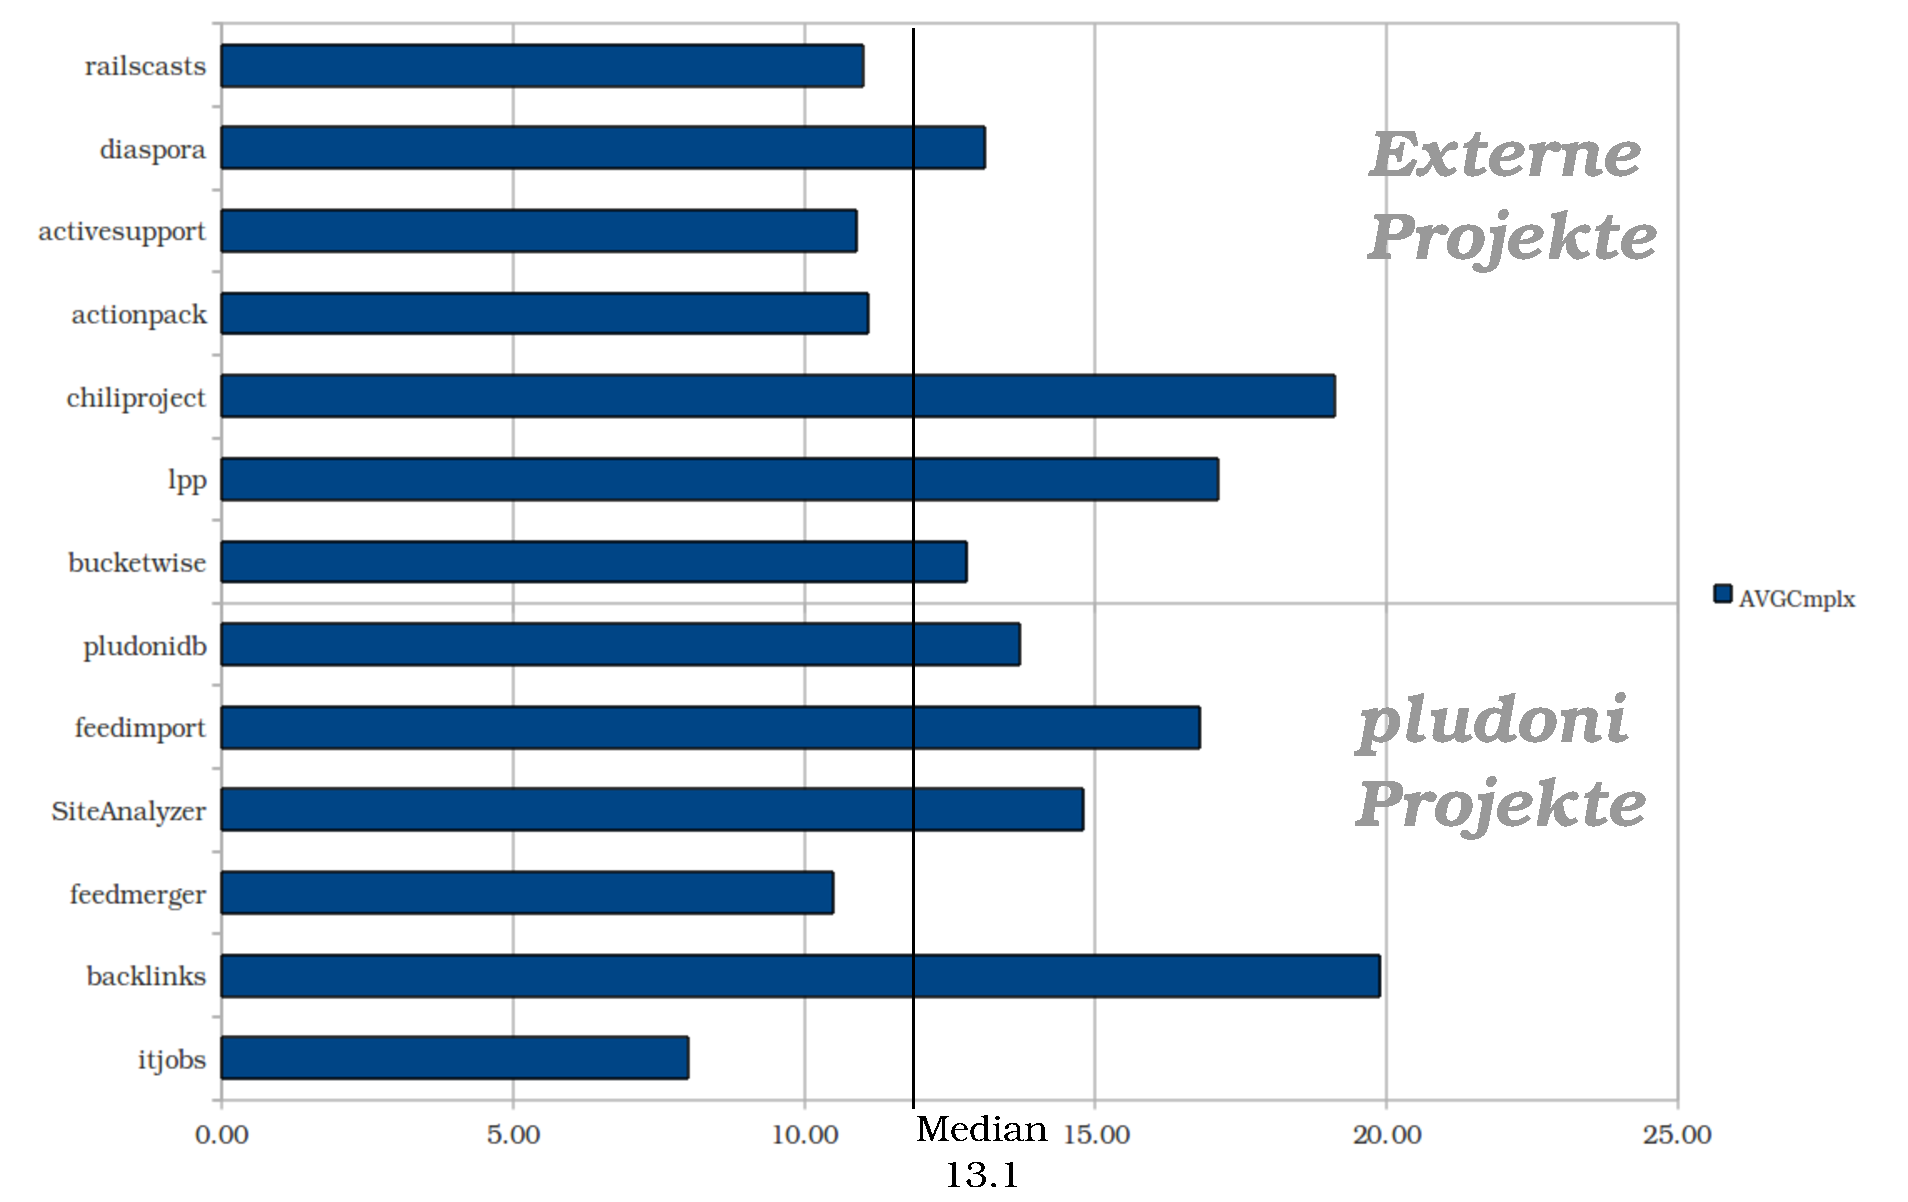
\includegraphics[width=\linewidth]{./diagrams/cmp-complex.pdf}
 % cpm-lotloc.pdf: 930x574 pixel, 72dpi, 32.81x20.25 cm, bb=0 0 930 574
 \caption{Vergleich der durchschnittlichen Komplexität}
 \label{fig:cpm-complex}
\end{figure}

\begin{figure}[hp]
 \centering
 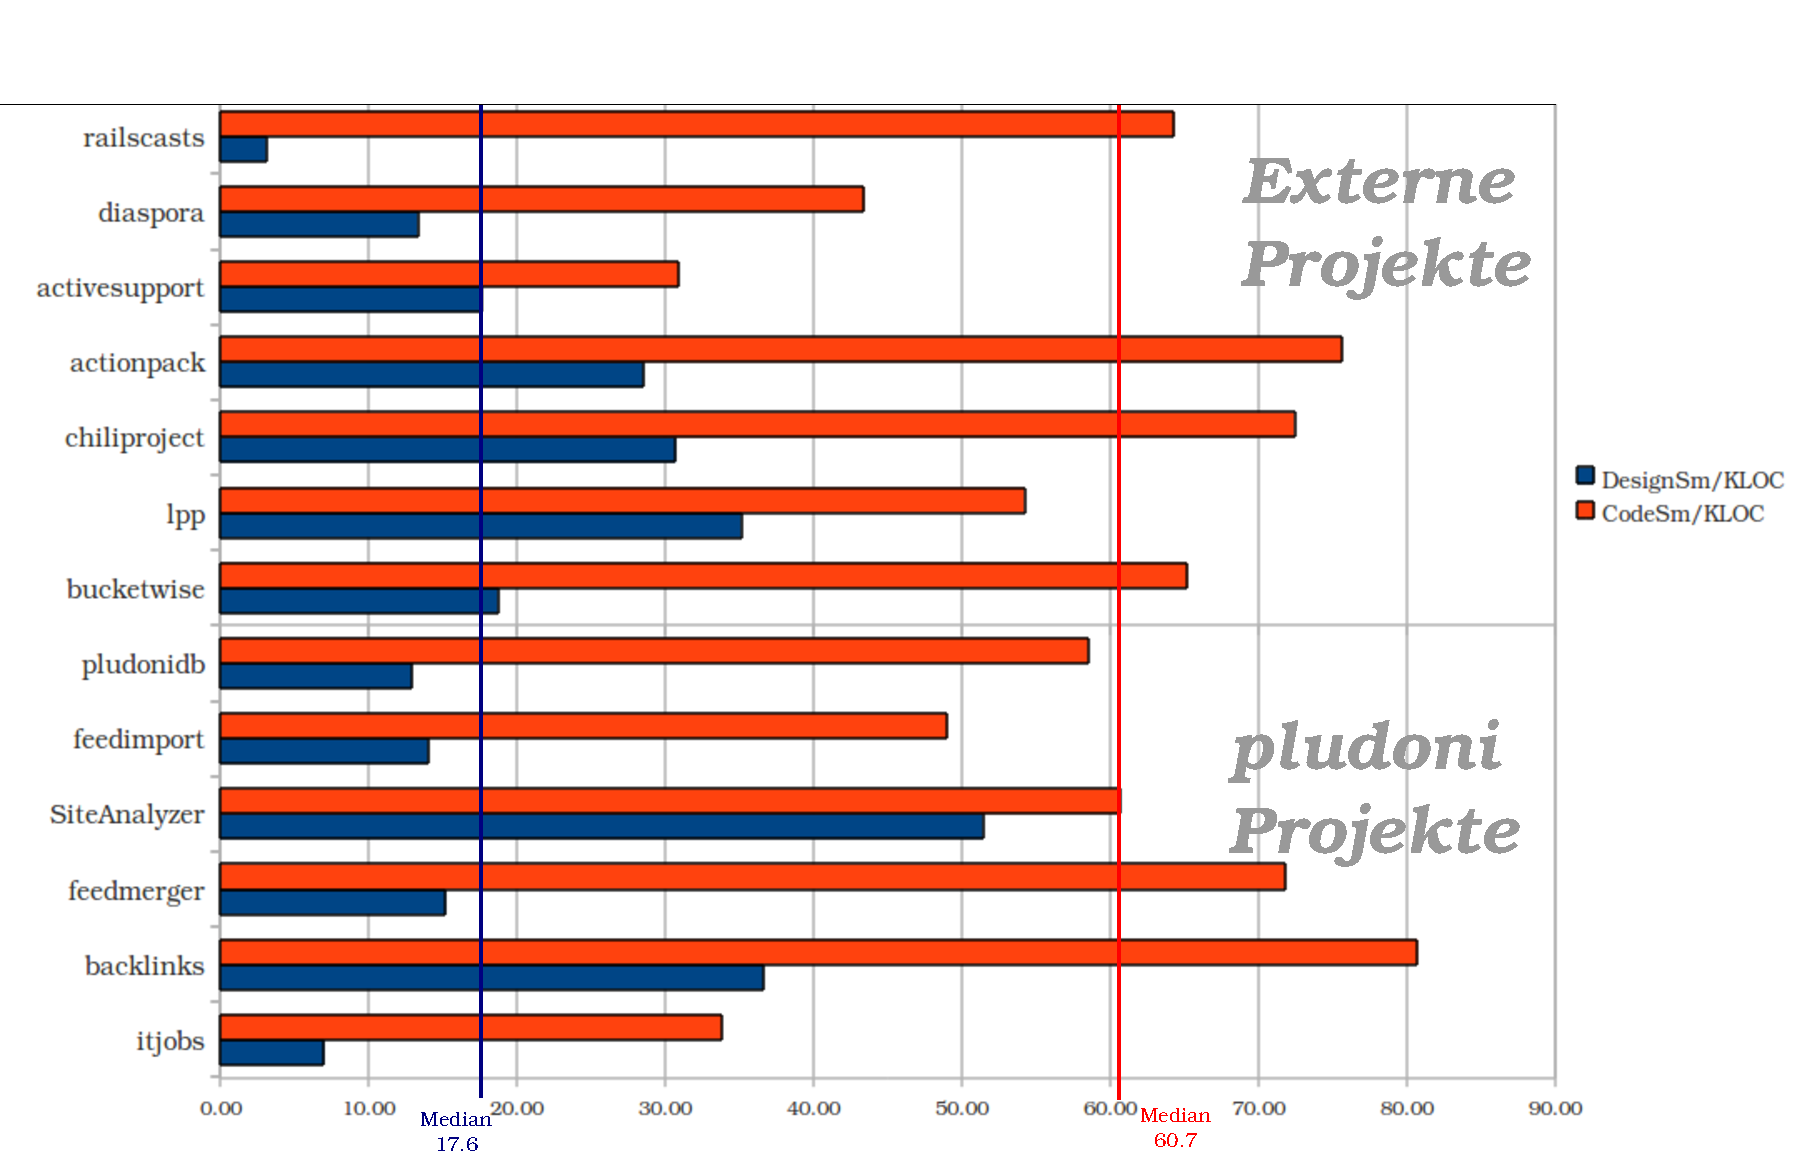
\includegraphics[width=\linewidth]{./diagrams/cpm-smells.pdf}
 % cpm-lotloc.pdf: 930x574 pixel, 72dpi, 32.81x20.25 cm, bb=0 0 930 574
 \caption{Vergleich der Anzahl Smells pro KLOC}
 \label{fig:cpm-complex}
\end{figure}

\subsection{Studien zu TDD}

Viele Studien belegen die positiven Effekte, die \glossar{TDD} für die Software-Entwicklung hat.

% Code Qualität

So zeigt eine Fallstudie, basierend auf einer Master Arbeit, dass TDD zu größerer Produktqualität bei gleichzeitigt hoher Flexibilität führt, was ebenso in einer höheren Zufriedenheit bei den Programmiern führt \citep{hans_wasmus_evaluation_2007}.


\marginnote{Empirische Untersuchung der Auswirkung auf Code-Qualität}Einer empirischen Studie von \citeauthor{madeyski_test-driven_2009} zufolge, sei TDD schwierg zu erlernen und in einigen Metriken (Klassen pro Methode, Development Speed, Anteil der bestandenen Akzeptanztests) nicht signifikant besser als traditionelle Test-Last-Methoden. Allerdings hatten die beteiligten TDD-geführten Projekte eine signifikant bessere Testabdeckung und geringere Kopplung unter den Klassen. Test-First sei letztendlich eine mächtige aber kontraintuitive Technik \citep{madeyski_test-driven_2009}.


In dem Artikel des IEEE-Software-Journals stellen \citeauthor{janzen_does_2008} eine Studie vor, die akademische und industrielle Javaprojekte die testgetrieben durchgeführt wurden (Test-First), mit denen, bei denen hinterher getestet wurde (Test-Last), vergleicht. Demnach zeigen die Ergebnisse an, dass Programmierer, die einen Test-First Ansatz verfolgen, tendenziell Software in kleineren Einheiten die weniger komplex sind, schreiben, als solche die erst nach der Entwicklung testen \citep{janzen_does_2008}.

\marginnote{Auswirkungen auf die Struktur -- Assignment Controllability}
Einer Studie von \citeauthor{mueller_effect_2006} zufolge, führt Testen im Allgemeinen zu weniger Methoden und geringerer Kopplung. Der Autor stellt auch eine potenzielle Metrik vor, um statistisch signifikant Projekte, die nach TDD betrieben wurden, von traditionellen Projekten zu unterscheiden: Assignment Controllability\footnote{Dies ist ein Maß, inwieweit der lokale Zustand einer Klasse/Methode von außen durch Parameter beeinflusst werden kann} \citep{mueller_effect_2006}. Allerdings rät der Autor zu weiteren Untersuchungen und setzt auch keinen Grenzwert an, ab welchem Grad der Controllability ein Projekt als TDD-Projekt bezeichnet werden kann.

% Verstaendnis
\marginnote{Verständnis von TDD in der Industrie}
Einer Umfrage unter 25 IT- und Entwicklungsleitern ergab, dass diese zwar die positiven Effekte unterstützen, aber nur 16\% TDD in der Praxis einsetzen, und nur 21\% Testvollständigkeit messen. Auch verstehen anscheinend etwa die Hälfte der Befragten den Begriff TDD falsch, nämlich als die reine Praxis Tests für alle denkbaren Problemfälle zu schreiben \citep{stelligent_inc_stelligent_2007}.

Das unter den Entwicklungsleitern der Fortune 500 Firmen, die von sich selbst behaupten, TDD zu betreiben, einige von Fehlannahmen ausgehen, wird in dem oben genannten Artikel genannt \citep{janzen_does_2008}. So setzen diese TDD mit automatisierten Tests gleich, oder behaupten sogar TDD sei das Schreiben ALLER Testfälle vor der Implementationsphase, anstelle der eigentlich gedachten kurzen Entwicklungs-Iterationen \citep{janzen_does_2008}.

% Auswirkungen auf Produktivit't und Bugs
\marginnote{Auswirkungen auf die Produktivität}
Einer Studie von Microsoft ergab, dass TDD-entwickelnde Teams eine 60\% -- 90\% geringere Fehlerdichte, aber eine 15\% -- 35\% längere Entwicklungszeit hätten, als nicht-TDD Entwickelnde \citep{nagappan_realizing_2008}.

















\subsection{Eigenschaften erfolgreicher Tests -- IN ARBEIT!!}

TODO Ueberarbeitung und merging mit MSDNA Tipps und eigene Erfahrungen
%TODO 

Das Vorhandensein von zahlreichen Tests reicht nicht, um das Testen erfolgreich abzuschließen. Zur Beurteilung der Brauchbarkeit einer Testsuite genügen die folgenden Kriterien \cite[S.272-279]{rappin_rails_2011}.



\begin{description}
 \item[Unabhängigkeit (Independence)] Ein Test ist unabhängig, falls er nicht durch andere Tests beeinflusst wird. Auch die Reihenfolge, in der die Tests ausgeführt werden, darf auf das Ergebnis keinen Einfluss üben. Siehe auch \citep{beck_test_2002}.
 \item[Wiederholbarkeit (Repeatability] Ein Test wird als wiederholbar bezeichnet, wenn er mehrmals hintereinander ausgeführt werden kann, und dabei jedes mal dasselbe Ergebnis liefert. Problematisch sind dabei z.B. Datum und Zeit, sowie Zufallsfunktionen
 \item[Klarheit (Clarity)] Ein Test ist klar, wenn sein Zweck sofort verständlich wird. Damit wird einerseits die Lesbarkeit gemeint. Anderseits schließt dies auch ein, ob der Test genau eine Eigenschaft testet und nicht redundant zu anderen Tests ist. Dies hat zur Folge, dass die Tests wartbarer werden und als Code Dokumenation dienen können.
 \item[Präzise (Conciseness)] Ein Test ist präzise, wenn er so wenig Code und so wenige Objekte wie möglich benötigt, um sein Ziel zu erreichen. Eine Auswirkung ist, dass der Test schneller wird.
 \item[Robustheit (Robustness)] Ein Test ist robust, wenn es eine direkte Korrelation zum zu testenden Code gibt: Ist der Code korrekt, so ist der Test erfolgreich. Ist der Code falsch, so schlägt der Test fehl. Nicht-robuste Tests werden auch "`zerbrechlich"' (brittle) genannt. Dazu zählen auch sogenannte tautologische Tests, die immer erfolgreich Verlaufen, und keine Aussage über den zugrunde liegenden Programmcode geben
 \end{description}

% Einige dieser Punkte können durch Metriken überprüft werden. Dazu mehr im Abschnitt \ref{sec:metrics}.
%  Code Craft S 144

  
  \subsection{Vorteile von TDD}
   
  Die Test-Suite, die durch TDD entsteht, kann als zusätzliche Dokumentation dienen, die nie veraltet, im Gegensatz zu einer geschriebenen Dokumentation \citep{palermo_guidelines_2006}.
  
  Die Software-Engineering Literatur ist sich einig, dass ein Bug teurer wird, je später er gefunden wird \citep{hunt_pragmatic_1999}[S. 238]. TDD hilft somit, einen Bug so frühzeitig wie möglich zu entdecken, und hat so das Potenzial, Budget einzusparen.
  
  Softwaresysteme, die durch TDD entstehen, tendieren dazu deutlich besser designt, lose gekoppelt und besser wartbar zu sein \citep{beck_test_2002} \citep{palermo_guidelines_2006}, da Refaktorisierungen mit hoher Zuversicht durchgeführt werden können
  
  Zusammenfassend führt TDD zu einer erhöhten Produktivität, da das Maß an manuellen Tests reduziert wird und Debuggen deutlich weniger wird \citep{palermo_guidelines_2006}.
  
  \subsection{Nachteile und Grenzen von TDD}
  Es gibt bestimmte Programmieraufgaben, die nicht allein durch die testgetriebene Entwicklung implementiert werden können. So seinen Nebenläufigkeit oder Software Sicherheit genannt, in denen TDD als Zielgeber nicht ausreiche \citep[S. xii]{beck_test_2002}.
  
  Zudem stelle die Testgetriebene Entwicklung kein Ersatz für andere Arten von Tests, wie Performanz/Stress und Usability-Test \citep[S. 86]{beck_test_2002}.
    % TODO Beispiel oder besser noch in die Auswertung
    
%     Darach’s Challenge
% Darach Ennis has thrown down a gauntlet for extending the reach of TDD. He says:
% For example, there are a lot of fallacies blowing around various engineering orga-
% nizations and amongst various engineers that this book could help to dispell and
% some of these are:
% •You can’t test GUIs automaticaly (eg: Swing, CGI, JSP/Servlets/Struts)
% •You can’t unit test distributed objects automaticaly (eg: RPC and Messaging
% style, or CORBA/EJB and JMS)
% •You can’t test-first develop your database schema (eg: JDBC?)
% •There is no need to test third party or code generated by external tools
% •You can’t test first develop a language compiler / interpreter from BNF to
% production quality implementation
% 
% 
% 
% 
% Microsoft Vorgehensweise:
% 
% Start TDD from the beginning of projects. Do not stop in the middle and claim it
% doesn’t work. Do not start TDD late in the project cycle when the design has already
% been decided and majority of the code has been written. TDD is best done
% incrementally and continuously.
% For a team new to TDD, introduce automated build test integration towards the second
% third of the development phase—not too early but not too late. If this is a “Greenfield”
% project, adding the automated build test towards the second third of the development
% schedule allows the team to adjust to and become familiar with TDD. Prior to the
% automated build test integration, each developer should run all the test cases on their
% own machine.
% Convince the development team to add new tests every time a problem is found, no
% matter when the problem is found. By doing so, the unit test suites improve during the
% development and test phases.
% Get the test team involved and knowledgeable about the TDD approach. The test team
% should not accept new development release if the unit tests are failing.
% Hold a thorough review of an initial unit test plan, setting an ambitious goal of having
% the highest possible (agreed upon) code coverage targets.
% Constantly running the unit tests cases in a daily automatic build (or continuous
% integration); tests run should become the heartbeat of the system as well as a means to
% track progress of the development. This also gives a level of confidence to the team
% when new features are added.
% Encourage fast unit test execution and efficient unit test design. Test execution speed is
% very important since when all the tests are integrated, the complete execution can
% become quite long for a reasonably-sized project and when using constant test
% executions. Tests results are important early and often; they provide feedback on the
% current state of the system. Further, the faster the execution of the tests the more likely
% developers themselves will run the tests without waiting for the automated build tests
% results. Such constant execution of tests by developers may also result in faster unit
% tests additions and fixes.
% Share unit tests. Developers’ sharing their unit tests, as an essential practice of TDD,
% helps identify integration issues early on.
% Track the project using measurements. Count the number of test cases, code coverage,
% bugs found and fixed, source code count, test code count, and trend across time, to
% identify problems and to determine if TDD is working for you.
% Check morale of the team at the beginning and end of the project. Conduct periodical
% and informal surveys to gauge developers’ opinions on the TDD process and on their
% willingness to apply it in the future.
